% =====================================================================
%  MSc paper -- Overleaf project
%  Authors: Abdelilah Agouni, Byan Hussein, Bilal Yousfi (supervisor)
%
%  HOW THIS PROJECT WORKS
%  - Each section is its own file in sections/. Write one section at a time.
%  - Lines starting with % are notes to you. They never appear in the PDF.
%  - \todo{...} prints red text in the PDF, so you can see what is unfinished.
%    Delete each \todo when the part is written.
%  - Cite with \cite{key}. Keys are in refs.bib (list at the bottom of this file).
%    Numbers [1], [2], ... are assigned automatically in order of first citation.
%  - Tables and figures are already in place with the verified numbers.
%    Refer to them with Table~\ref{tab:main} or Fig.~\ref{fig:size}.
%  - Compiler: pdfLaTeX (Overleaf default). Bibliography: biber (automatic).
% =====================================================================

% IEEE two-column layout. If the target journal gives its own template,
% copy the sections/ folder and refs.bib into that template instead.
\documentclass[conference]{IEEEtran}

\usepackage[utf8]{inputenc}
\usepackage[T1]{fontenc}
\usepackage{amsmath,amssymb}
\usepackage{graphicx}
\usepackage{booktabs}
\usepackage{array}
\usepackage{xcolor}
\usepackage{tikz}
\usetikzlibrary{arrows.meta,positioning,shapes.geometric,calc,patterns}
\usepackage[hidelinks]{hyperref}
\usepackage[style=ieee,doi=true,url=false,isbn=false,eprint=false,backend=biber]{biblatex}
\addbibresource{refs.bib}

\graphicspath{{figures/}}

% Red marker for unfinished parts. Delete each \todo when you write that part.
\newcommand{\todo}[1]{\textcolor{red}{[TODO: #1]}}

% Consistent names (change here once, it changes everywhere)
\newcommand{\RA}{Route~A}
\newcommand{\RB}{Route~B}
\newcommand{\Aclean}{A-clean}

\begin{document}

% ---------------------------------------------------------------------
% TITLE -- agree the final title with Dr. Yousfi.
% Current title (thesis version):
\title{When Is Self-Similarity Enough? Defect Size and Reference
Contamination in Zero-Shot Texture Anomaly Detection}
% Option recommended for the paper (states the result, keyword-rich):
% \title{Large Defects Contaminate Their Own Reference: Limits of Mean
% Self-Similarity in Zero-Shot Texture Anomaly Detection}
% Option keeping the question:
% \title{When Is Mean Self-Similarity Enough? Defect Size and Reference
% Contamination in Zero-Shot Texture Anomaly Detection}
% ---------------------------------------------------------------------

\author{
\IEEEauthorblockN{Abdelilah Agouni, Byan Hussein, Bilal Yousfi}
\IEEEauthorblockA{Department of Computer Engineering, Faculty of \todo{faculty name}\\
Karab\"uk University, Karab\"uk, T\"urkiye\\
Corresponding author: abdelilah.agouni@gmail.com}
}

\maketitle


% PART 1 (requested by Dr. Yousfi): Introduction, Literature Review, Methodology.
% Remove the % in front of a line to add that part to the PDF later.
% \begin{abstract}
% WRITE THIS LAST (course PDF, slide 81: "introduction and abstract last").
% Limit: 250 words. One paragraph. No citations.
% Structure, one or two sentences each:
%   1. Context: zero-shot texture detectors compare a patch with the rest of
%      the same image, so they assume most of the image is normal.
%   2. Gap: nobody measured how this fails as defects grow.
%   3. What you did: Route A vs Route B (4 clean photos) vs FCA, frozen DINOv2,
%      five MVTec AD textures, 382 defective images.
%   4. Results WITH numbers: Pixel AP 32.1 -> 50.0; slope difference -2.72
%      [-3.49, -1.93]; FCA not steeper than Route B; A-clean recovers about
%      half (real) and two thirds (synthetic) of the slope.
%   5. Conclusion: the size dependence belongs to the simple mean reference.
% Define every abbreviation the first time (AUROC, AP, AU-PRO, FCA).
\todo{Write the abstract last (max 250 words).}
\end{abstract}

\begin{IEEEkeywords}
Texture anomaly detection, zero-shot learning, few-shot learning, DINOv2,
defect size, reference contamination, MVTec AD
\end{IEEEkeywords}
     % write last
\section{Introduction}
\label{sec:intro}
% The authors' introduction (Nov 20), with the corrections accepted.
% Keep editing it in your own words.

Textured products such as carpet, leather, wood and tile are judged by their
appearance, so even a small defect can make them unsellable. Industry needs
computers and software to do visual inspection and to check every product on
the production line. Companies mostly produce good products, so if we wait to
collect hundreds of images of defective products, it takes a long time. Also,
inspection by human workers is slow, and they miss small defects when they
become tired.

Defects are also varied, and labelling is very expensive, because the exact
defect must be drawn pixel by pixel. Instead of learning what defects look
like, methods therefore learn what normal products look like and flag anything
different. This approach is called anomaly detection (AD), and the MVTec AD
dataset is its standard benchmark~\cite{bergmann2021mvtec}.

Training-free AD methods differ mainly in where they find their reference for
``normal''. Zero-shot single-image methods use no reference images at all: they
only compare each patch of the test image with the rest of the same image and
flag regions that break its homogeneity~\cite{aota2023zeroshot,ardelean2024highfidelity,yao2025grnr,zhang2025nlpa}.
Few-shot methods build a memory bank from the patches of a few defect-free
reference images and give each test patch a score from its distance to the
nearest entry~\cite{roth2022patchcore,damm2025anomalydino,lendering2026subspacead}.

Batched zero-shot methods compare patches across many unlabelled test
images~\cite{li2024musc,legia2025consistent}. Frozen self-supervised features,
in particular DINOv2~\cite{oquab2024dinov2}, make all three families practical
without any training.

Single-image methods depend on an assumption: most of the image is normal.
Aota et~al.~\cite{aota2023zeroshot} state this assumption for pixel-level
detection, and the authors of feature correspondence analysis
(FCA)~\cite{ardelean2024highfidelity} acknowledge a limitation when anomalies
extend across most of the image. The underlying assumption is therefore
expected to become less reliable as defect size increases, because a large
defect becomes part of the reference that each patch is compared with.
Published results, however, are reported as averages over all defects, which
hides any dependence on size. Defect size has been studied for a single method
and small defects~\cite{lehr2024limitations}, and contamination of the
reference set of few-shot detectors has been studied~\cite{villanueva2026cleaning},
but to our knowledge no study has measured how single-image self-similarity and
a few-shot memory bank compare across defect sizes on the same frozen features,
or tested whether the defect contaminating the image's own reference explains
the difference.
% NOTE: confirm "to our knowledge" with Google Scholar and arXiv
% (strings G1--G3 in the workbook) before submission.

This study fills that gap with four research questions:
\begin{enumerate}
  \item[RQ1:] How much does a four-image memory bank improve on a simple
  mean-similarity single-image baseline?
  \item[RQ2:] How does that improvement depend on defect size?
  \item[RQ3:] How much of the size dependence comes from the defect
  contaminating the image's own reference?
  \item[RQ4:] Does a robust published single-image method (FCA) show the same
  dependence?
\end{enumerate}

We do not propose a new detector. We compare a mean-similarity single-image
baseline (Route~A), our implementation of the memory-bank idea of
AnomalyDINO~\cite{damm2025anomalydino} (Route~B) and the official FCA code on
the five MVTec AD textures, with the same frozen DINOv2 features and the same
metric code.

The main contributions of this work are as follows:
\begin{enumerate}
  \item A controlled comparison of references. On the same frozen DINOv2
  features and with the same metric code, we show that a four-image memory bank
  outperforms mean self-similarity on all five textures (pixel-level average
  precision, Pixel AP, 32.1\% vs.\ 50.0\%), and that a robust published
  single-image method (FCA) outperforms both on segmentation.
  \item A size analysis. On 382 defective images, we show that the advantage of
  the memory bank grows with defect size (a slope difference of $-2.72$ points
  of per-image area under the ROC curve, AUROC, per unit of log defect area),
  while the slope of FCA cannot be distinguished from that of the memory bank;
the strong size dependence is therefore not shared by every single-image
method.
  \item An intervention study. On real and synthetic defects, we show that
  removing the defect from the image's own reference recovers about half of the
  size slope on real defects and about two thirds on synthetic defects, whereas median and trimmed-mean references recover little; on real defects
the rest of the slope remains unexplained.
\end{enumerate}
We also report the ideas that did not work (routing between the two methods, an
image-level mean score and feature drift), and we fixed every success criterion
before running the analysis; code and results are kept in a tagged repository that will be made public
on publication.

The rest of this paper is organised as follows.
Section~\ref{sec:related} reviews the related literature and
Section~\ref{sec:methods} describes the methodology; Section~IV presents the
results, Section~V discusses them and Section~VI concludes.
% When Results, Discussion and Conclusion are switched on in main.tex,
% replace IV, V, VI with \ref{sec:results}, \ref{sec:discussion}, \ref{sec:conclusion}.

\section{Literature Review}
\label{sec:related}
% Draft for the authors to review and rewrite in their own words.
% Every claim below is checked against the literature matrix
% (paper_literature_and_course_checklist.xlsx, sheet "Literature matrix").

\subsection{Industrial anomaly detection and MVTec AD}
MVTec AD~\cite{bergmann2021mvtec} contains defect-free training images and
annotated test images for 15 categories, five of which are textures:
carpet, grid, leather, tile and wood. Most recent methods are evaluated on
it with image-level and pixel-level area under the receiver operating
characteristic curve (AUROC) and the per-region overlap (PRO). Because the
test pixels are overwhelmingly normal (about 97\% on MVTec
AD~\cite{li2024musc}), pixel AUROC is lenient, and studies increasingly
report pixel-level average precision (AP) and the area under the PRO curve
(AU-PRO) as well.

\subsection{Zero-shot single-image methods}
Aota et~al.~\cite{aota2023zeroshot} showed that texture anomalies can be
detected without any normal training images. Their method uses all patches
of the test image as the gallery and scores each patch by its mean distance
to its $K$ nearest neighbours ($K=400$ of 1{,}600 patches), using
WideResNet-50 features at $320\times320$ pixels. The method assumes that
normal regions form the majority of the image, and it is insensitive to the
orientation mismatch between training and test images that hurts many-shot
methods. FCA~\cite{ardelean2024highfidelity} replaces the nearest-neighbour
score with a comparison of local feature statistics against a median
reference, using a one-dimensional Wasserstein correspondence, and reports a
large reduction in localisation error on the MVTec AD textures; its
supplementary material notes failures when the anomaly covers the majority
of the image. Global-regularized neighborhood regression
(GRNR)~\cite{yao2025grnr} reconstructs each query from its neighbourhood with
a global normality prior, and NLPA-AD~\cite{zhang2025nlpa} propagates normal
labels across the texture while stopping propagation at likely anomalous
points. INP-Former~\cite{luo2025inp} learns to extract normal prototypes from
the test image itself, but it requires training. All of these methods take
their reference from the test image and report averages over all defects.

\subsection{Few-shot memory banks}
PatchCore~\cite{roth2022patchcore} introduced a memory bank of nominal patch
features from the full training set, scored by nearest-neighbour distance. AnomalyDINO~\cite{damm2025anomalydino}
showed that frozen DINOv2 patch features~\cite{oquab2024dinov2} make this
idea strong in the few-shot regime: with a memory bank built from a handful
of reference images and cosine distance to the nearest patch, it raised
one-shot image AUROC on MVTec AD from 93.1\% to 96.6\% without training.
SubspaceAD~\cite{lendering2026subspacead} models few-shot DINOv2 features
with a principal-component subspace and reports a PRO of about 97\% on the
textures with four references. Few-shot methods do not depend on the test
image being mostly normal, but they assume that the references are clean;
replacing three of ten references with defective images costs 1.8 AUROC points on average over four datasets (1.3 on MVTec AD)~\cite{villanueva2026cleaning}.

\subsection{Batched zero-shot methods}
MuSc~\cite{li2024musc} scores each patch against the patches of all other
unlabelled test images and aggregates local neighbourhoods at several scales,
small for small defects and large for large ones. Le-Gia and
Ahn~\cite{legia2025consistent} show that such methods fail when the same
anomaly recurs across test images, and they observe that these consistent
anomalies often have large masks. Batched methods need many test images at
once, which differs from the single-image setting studied here.

\subsection{Defect size and contamination}
Defect size has received little direct attention. Lehr
et~al.~\cite{lehr2024limitations} grow a defect pattern in steps and
measure the smallest reliably detected size for one method. The
contamination studied for few-shot detectors concerns defective images in
the reference set~\cite{villanueva2026cleaning}, not a defect inside the
test image that becomes part of its own reference.

\subsection{Summary and research gap}
Table~\ref{tab:lit} summarises where each family takes its reference. The
literature establishes that single-image methods assume a majority of
normal patches~\cite{aota2023zeroshot,ardelean2024highfidelity}, but it
reports results as averages over all defects. To our knowledge, no study has
compared a single-image and a few-shot reference across defect sizes on the
same features, or tested with an intervention whether contamination of the
image's own reference explains the difference. This is an empirical gap
(the size dependence has not been measured) and a methodological gap
(average scores cannot reveal it).

\begin{table}[t]
\centering
\caption{Where training-free texture anomaly detectors take their reference
for ``normal''.}
\label{tab:lit}
\footnotesize
\setlength{\tabcolsep}{3pt}
\begin{tabular}{>{\raggedright\arraybackslash}p{2.0cm}>{\raggedright\arraybackslash}p{1.5cm}>{\raggedright\arraybackslash}p{4.3cm}}
\toprule
Family & Examples & Reference and assumption \\
\midrule
Zero-shot, single image & \cite{aota2023zeroshot,ardelean2024highfidelity,yao2025grnr,zhang2025nlpa}
  & Rest of the test image; most of the image is normal \\
Memory bank (few-shot) & \cite{roth2022patchcore,damm2025anomalydino,lendering2026subspacead}
  & Patches of a few clean images; references are clean \\
Batched zero-shot & \cite{li2024musc,legia2025consistent}
  & Other unlabelled test images; anomalies do not recur \\
\bottomrule
\end{tabular}
\end{table}
   % Literature Review
\section{Methodology}
\label{sec:methods}
% Draft for the authors to review and rewrite in their own words.
% All settings below match the committed code (tag v1.0-results).

Fig.~\ref{fig:pipeline} summarises the approach. Every test image is passed
through the same frozen feature extractor; the methods differ only in the
reference against which each patch is compared. We then evaluate the
anomaly maps with one metric code, analyse how per-image accuracy depends on
defect size, and test the cause with interventions on the reference.

\begin{figure*}[t]
\centering
% Vector figure built from figures/method_overview.tex (see method_overview_standalone.tex)
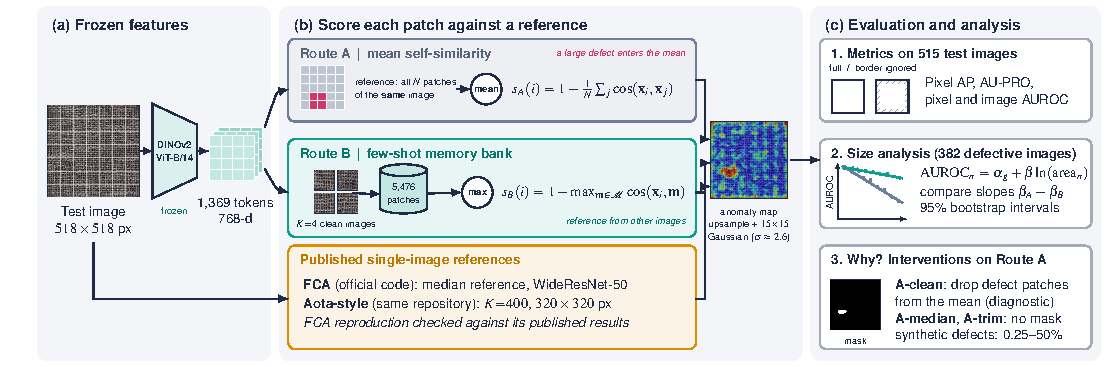
\includegraphics[width=\textwidth]{method_overview.pdf}
\caption{Overview of the methodology. (a)~Each test image is encoded once by a
frozen DINOv2 ViT-B/14 into 1{,}369 patch tokens. (b)~Each patch is scored
against a reference: Route~A uses all patches of the same image, so a large
defect enters its mean; Route~B uses a memory bank built from four clean images;
FCA runs with its official code and the Aota-style variant with the
reimplementation in the same repository, each with its own features. (c)~All anomaly maps are evaluated with one metric code on two
protocols, per-image accuracy is regressed on log defect area, and
interventions on Route~A's reference test the cause. The thumbnails show a
carpet test image, its ground-truth mask and its Route~A map; the reference
tiles are illustrative.}
\label{fig:pipeline}
\end{figure*}

\subsection{Dataset and evaluation protocol}
We use the five texture categories of MVTec AD~\cite{bergmann2021mvtec}:
carpet, grid, leather, tile and wood, with 117, 78, 124, 117 and 79 test
images (515 in total: 133 defect-free and 382 defective). Thirty training
images per category are loaded from the official training split; they serve
only as the pool for Route~B's references. Images are resized to
$518\times518$ pixels.

We report four metrics per texture and their five-texture average:
pixel-level average precision (Pixel AP), the area under the per-region
overlap curve (AU-PRO; 1{,}000 thresholds, integrated up to a false-positive
rate of 0.3 and normalised), pixel AUROC, and image AUROC, for which the
image score is the maximum of the anomaly map. Aota et~al.~\cite{aota2023zeroshot} evaluate on a centre crop that removes
about 10\% of each side, so every result is reported on two protocols: the full image, and a cropped protocol
that ignores a 52-pixel border (about 10\%) of both the map and the mask. Two
defective images (one in grid, one in tile) have their defect entirely inside
this border; they are dropped from the cropped size analysis ($n=380$).

\subsection{Feature extraction}
Both routes use DINOv2 ViT-B/14~\cite{oquab2024dinov2} without any training.
A $518\times518$ input gives a $37\times37$ grid of $N=1{,}369$ patch
tokens of dimension 768, taken from the final block, stored at half precision (fp16) and
L2-normalised. Each
patch score map is upsampled bilinearly to $518\times518$ and smoothed with a
$15\times15$ Gaussian filter (OpenCV, with $\sigma$ derived from the kernel
size, about 2.6 pixels). The main results use the final block; a sweep over
blocks 6, 8, 10, 12 and the mean of blocks 7--9 tests this choice.

\subsection{Route A: single-image mean similarity}
Route~A compares each patch $\mathbf{x}_i$ with all patches of the same
image and uses the mean cosine similarity as its reference:
\begin{equation}
  s_A(i) = 1 - \frac{1}{N}\sum_{j=1}^{N} \cos(\mathbf{x}_i,\mathbf{x}_j).
  \label{eq:routeA}
\end{equation}
A patch that differs from the image as a whole receives a high score. If a
defect covers a large share of the image, however, the defect patches enter
the mean in~\eqref{eq:routeA} and pull the reference towards the defect; this
is the contamination we test in Section~\ref{sec:interventions}.

\subsection{Route B: few-shot memory bank}
Route~B follows the memory-bank idea of AnomalyDINO~\cite{damm2025anomalydino}.
The memory bank $\mathcal{M}$ holds the $4\times1{,}369=5{,}476$ patches of
$K=4$ defect-free reference images, drawn at random by seed from the 30
loaded training images. Each test patch is scored by its distance to the
nearest entry:
\begin{equation}
  s_B(i) = 1 - \max_{\mathbf{m}\in\mathcal{M}} \cos(\mathbf{x}_i,\mathbf{m}).
  \label{eq:routeB}
\end{equation}
Because the reference comes from other images, a defect in the test image
cannot contaminate it. The main results use seeds 42, 123 and 2026. The size analysis
uses seed 42, the interventions on real defects use the mean of ten seeds,
and the synthetic experiments use five seeds. Route~B differs from AnomalyDINO in backbone
size, resolution, smoothing, the absence of rotation augmentation and the
image-level score, so we do not call it AnomalyDINO.

\subsection{Published single-image references}
To test whether any size dependence is specific to Route~A, we run the
official FCA code~\cite{ardelean2024highfidelity} (commit \texttt{afe8326},
MIT licence) at full resolution. Before computing any new result we checked
the reproduction: the published per-texture PRO and pixel AUROC are matched
within 0.01 points on all five textures. The repository pins Python 3.9 and
PyTorch 2.1.2; we ran it with Python 3.13 and PyTorch 2.6.0, with two small
wrapper fixes for file input and output and no change to the method. We also run the repository's
reimplementation of Aota et~al.~\cite{aota2023zeroshot} at $320\times320$
pixels with a $3\times3$ tile and $K=400$. Both sets of maps are rescaled to
the $518\times518$ grid and scored with our metric code.

\subsection{Size analysis}
For each defective image $n$ we compute its pixel AUROC, which does not
depend on how many pixels are defective, and regress it on the natural
logarithm of the defect area (pixels on the $518\times518$ grid):
\begin{equation}
  \mathrm{AUROC}_n = \alpha_{g(n)} + \beta \ln(\mathrm{area}_n) + \varepsilon_n ,
  \label{eq:slope}
\end{equation}
where $\alpha_{g(n)}$ is a fixed effect for each texture--defect-type group
(25 groups), so that the slope $\beta$ is estimated within groups. One unit
of $\ln(\mathrm{area})$ corresponds to multiplying the area by $e\approx2.7$,
and $\beta$ is expressed in AUROC points per unit. A more negative slope means
that accuracy falls faster as defects grow. We compare methods through the
slope difference on the same images (for example $\beta_A-\beta_B$), with
95\% confidence intervals from 10{,}000 bootstrap resamples of images. To
check that a smaller slope is not only a ceiling effect near an AUROC of
100, we also regress the log ratio of the two methods' errors
($100-\mathrm{AUROC}$) on log area.

\subsection{Interventions on the reference}
\label{sec:interventions}
To test whether the defect contaminates Route~A's reference, we change only
the reference in~\eqref{eq:routeA}:
\begin{itemize}
  \item \textbf{A-clean} takes the mean over non-defect patches only, using
  the ground-truth mask. It is a diagnostic, not a deployable method.
  \item \textbf{A-median} replaces the mean by the median of the similarities.
  \item \textbf{A-trim} replaces it by a mean that drops the lowest 25\% of
  the similarities.
\end{itemize}
If contamination drives the size dependence, A-clean should remove much of
Route~A's slope, while the two mask-free variants show how much a simple
robust statistic recovers. We also compute a contamination index, the
distance between the mean feature of the whole image and the mean feature of
its non-defect patches.

\subsection{Synthetic defects}
Real defects do not allow size to be varied independently of content.
We therefore paste synthetic defects into the 133 defect-free test images:
irregular single-component blobs filled with a crop of another texture,
Gaussian noise ($\sigma=8$ grey levels), blur ($\sigma=8$ pixels) or a hue
shift of $60^\circ$ with brightness reduced to 65\% (on the greyscale grid
images only the darkening applies), at ten area fractions from 0.25\% to
50\%. Bootstrap resampling is over the 133 base images, because the copies of
one image are not independent. The key test compares 25\% with 50\% coverage:
once the defect is half of the image, a contaminated mean reference should
fail, while A-clean should not.

\subsection{Pre-set criteria and implementation}
For each analysis we fixed the success criterion before running it, and we
report every outcome, including negative ones. Two deviations are disclosed:
the 25\% coverage was added in a second run, because the first sweep
contained 32\% but not 25\% (in that first sweep the test held against 32\%
but not against 0.25\%, and we report both); and the drift criterion did not
specify the expected sign of its coefficient: drift met it, but with the
opposite sign to our hypothesis, so we do not treat drift as a mechanism. All experiments ran on a laptop with an
NVIDIA RTX 3050 GPU (4~GB), Python 3.13, PyTorch 2.6.0 and CUDA 12.4. Code,
configuration and results are kept in a git repository (release tag
\texttt{v1.0-results}).
        % Methodology
% \section{Results}
\label{sec:results}
% Course PDF: results = findings, WITHOUT interpretation (that goes in the
% Discussion). Every table and figure must be mentioned in the text.
% All numbers below are verified against the result files.

\subsection{Main comparison}
% Key points: Route B beats Route A on every texture and metric (full image):
% Pixel AP 32.1 -> 50.0 (+17.9), AU-PRO 86.6 -> 94.9, image AUROC 87.0 -> 99.8.
% Border ignored: gain shrinks (+7.5 Pixel AP). FCA is ahead of Route B on all
% segmentation metrics. Aota-style image AUROC 39.0 -> 99.3 once the border is
% ignored (border artefact).
\todo{Describe Table~\ref{tab:main} and Fig.~\ref{fig:pixelap}.}

\begin{table}[t]
\centering
\caption{Five-texture averages (\%), full image (F) and with a 10\% border
ignored (C). \RB: mean of three seeds. Last DINOv2 layer.}
\label{tab:main}
\footnotesize
\setlength{\tabcolsep}{3pt}
\begin{tabular}{llcccc}
\toprule
Method & Prot. & Pixel AP & AU-PRO & Pix.\ AUROC & Img.\ AUROC \\
\midrule
\RA & F & 32.1 & 86.6 & 92.1 & 87.0 \\
\RA & C & 43.8 & 89.1 & 94.1 & 91.3 \\
\RB & F & 50.0 & 94.9 & 97.0 & 99.8 \\
\RB & C & 51.3 & 93.2 & 97.1 & 99.9 \\
FCA \cite{ardelean2024highfidelity} & F & 70.4 & 95.9 & 98.1 & 97.1 \\
FCA \cite{ardelean2024highfidelity} & C & 76.8 & 97.1 & 98.8 & 99.5 \\
Aota-style \cite{aota2023zeroshot} & F & 26.3 & 83.8 & 93.4 & 39.0 \\
Aota-style \cite{aota2023zeroshot} & C & 66.5 & 95.9 & 98.2 & 99.3 \\
\bottomrule
\end{tabular}
\end{table}

\begin{figure}[t]
\centering
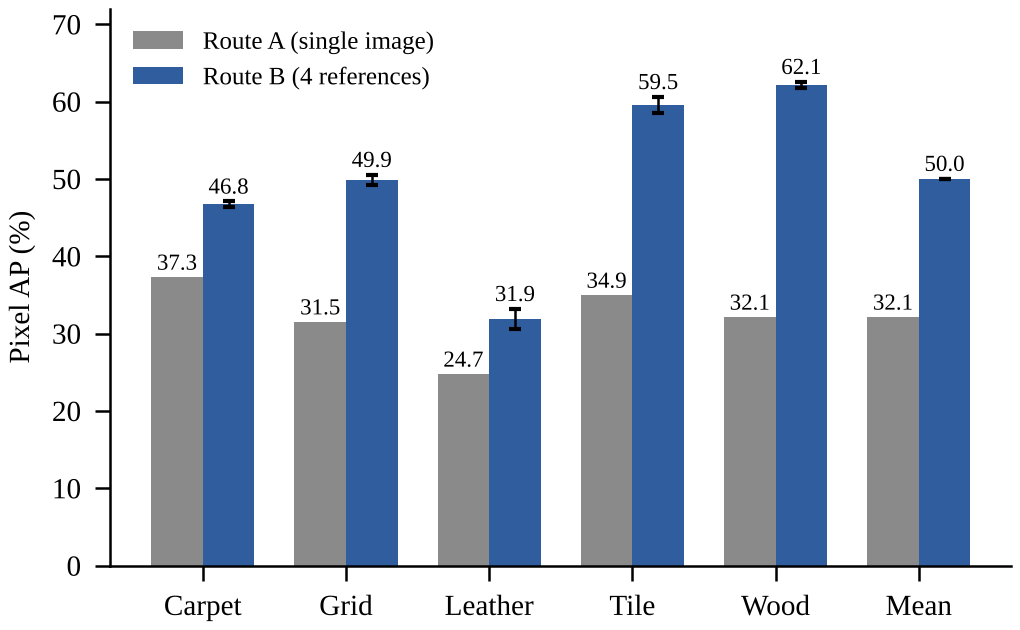
\includegraphics[width=\columnwidth]{fig1_pixel_ap_per_texture.png}
\caption{Pixel AP per texture, \RA\ versus \RB\ (full image). \RB: mean of
three seeds; bars show the standard deviation.}
\label{fig:pixelap}
\end{figure}

\subsection{Size dependence}
% Key points: slopes on log area: A -3.89, Aota-style -1.88, B -1.17,
% FCA -0.80 (full image). A - B = -2.72 [-3.49, -1.93]; FCA - B = +0.37
% [-0.19, +1.08], so FCA is not steeper than B. Per texture, Spearman between
% B's advantage and area is +0.49 to +0.70. Ceiling check: the log ratio of
% A's to B's error rises with area (+0.16 [+0.03, +0.29]).
\todo{Describe Table~\ref{tab:slopes} and Fig.~\ref{fig:size}.}

\begin{table}[t]
\centering
\caption{Slope of per-image pixel AUROC on log defect area (points), with
95\% intervals. \RB: seed 42. Full image $n=382$; border ignored $n=380$.}
\label{tab:slopes}
\footnotesize
\setlength{\tabcolsep}{4pt}
\begin{tabular}{lcc}
\toprule
Method & Full image & Border ignored \\
\midrule
\RA & $-3.89$ [$-5.48$, $-2.53$] & $-2.53$ [$-3.98$, $-1.52$] \\
Aota-style \cite{aota2023zeroshot} & $-1.88$ [$-3.02$, $-0.85$] & $-0.93$ [$-1.69$, $-0.37$] \\
\RB & $-1.17$ [$-2.14$, $-0.48$] & $-1.06$ [$-1.81$, $-0.56$] \\
FCA \cite{ardelean2024highfidelity} & $-0.80$ [$-1.32$, $-0.34$] & $-0.34$ [$-0.78$, $+0.01$] \\
\midrule
A $-$ B & $-2.72$ [$-3.49$, $-1.93$] & $-1.47$ [$-2.30$, $-0.85$] \\
FCA $-$ B & $+0.37$ [$-0.19$, $+1.08$] & $+0.72$ [$+0.27$, $+1.25$] \\
\bottomrule
\end{tabular}
\end{table}

\begin{figure}[t]
\centering
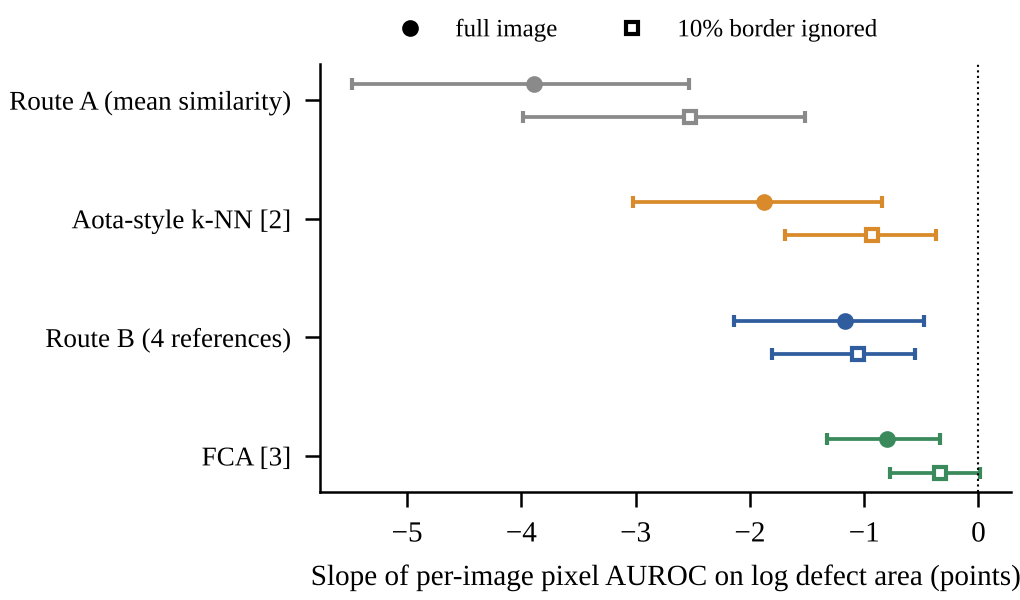
\includegraphics[width=\columnwidth]{fig2_size_slopes_real.png}
\caption{Slope of per-image pixel AUROC on log defect area on real defects,
with 95\% bootstrap intervals (filled: full image; open: 10\% border
ignored). \RB: seed 42.}
\label{fig:size}
\end{figure}

\subsection{Does contamination explain it?}
% Key points: A-clean - A = +1.96 [+1.28, +2.66] on real defects (about half
% of A's -3.89), +5.68 on synthetic (about two thirds of -8.56). A-median
% +0.19 (interval includes 0), A-trim +0.10. On real defects A-clean is still
% steeper than B (-0.75 [-1.14, -0.36]). Contamination index rises with area
% (pooled Spearman 0.96). At 25% -> 50% coverage: A -26.1 [-26.8, -25.4],
% A-clean -0.2 [-0.6, +0.2], in all four defect types (hue shift A-clean -1.3,
% inside the pre-set 2-point tolerance).
\todo{Describe Table~\ref{tab:contam}, Fig.~\ref{fig:realsyn} and Fig.~\ref{fig:coverage}.}

\begin{table}[t]
\centering
\caption{Effect of the reference on the size slope (points per unit of log
area; differences with 95\% intervals). $^\dagger$Uses the ground-truth mask.
\RB: ten seeds (real), five (synthetic).}
\label{tab:contam}
\footnotesize
\setlength{\tabcolsep}{4pt}
\begin{tabular}{lcc}
\toprule
Quantity & Real defects & Synthetic \\
\midrule
Slope of A & $-3.89$ & $-8.56$ \\
Slope of \Aclean$^\dagger$ & $-1.93$ & $-2.88$ \\
Slope of B & $-1.18$ & $-4.23$ \\
\midrule
\Aclean\ $-$ A & $+1.96$ [$+1.28$, $+2.66$] & $+5.68$ [$+5.57$, $+5.79$] \\
A-median $-$ A & $+0.19$ [$-0.05$, $+0.46$] & $+0.94$ [$+0.85$, $+1.03$] \\
A-trim $-$ A & $+0.10$ [$+0.03$, $+0.17$] & $+0.24$ [$+0.21$, $+0.28$] \\
\Aclean\ $-$ B & $-0.75$ [$-1.14$, $-0.36$] & $+1.35$ [$+1.25$, $+1.44$] \\
\bottomrule
\end{tabular}
\end{table}

\begin{figure}[t]
\centering
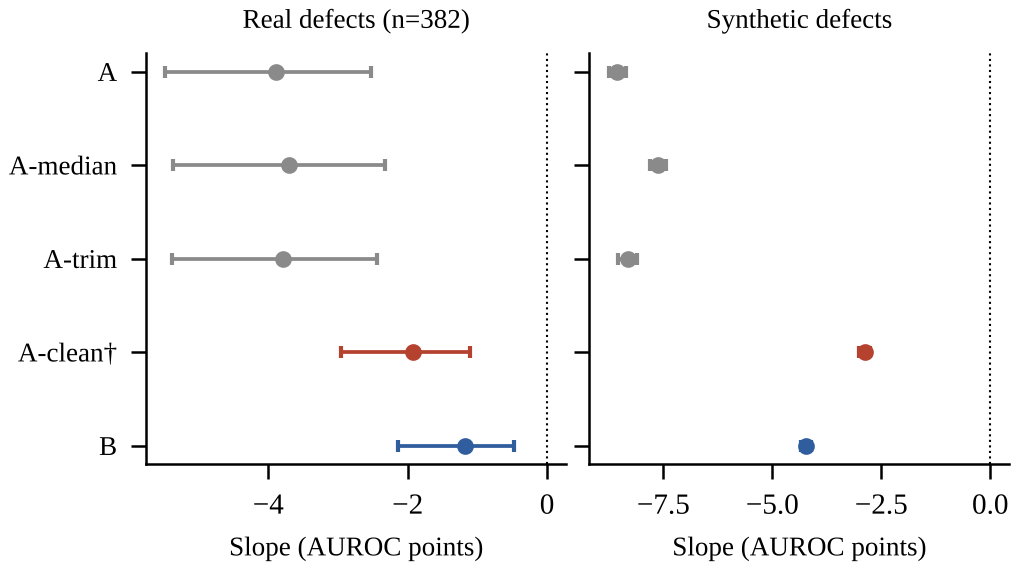
\includegraphics[width=\columnwidth]{fig3_slopes_real_vs_synthetic.png}
\caption{Slopes of per-image pixel AUROC on log area with 95\% intervals,
real and synthetic defects. $^\dagger$\Aclean\ uses the ground-truth mask
(diagnostic only).}
\label{fig:realsyn}
\end{figure}

\begin{figure}[t]
\centering
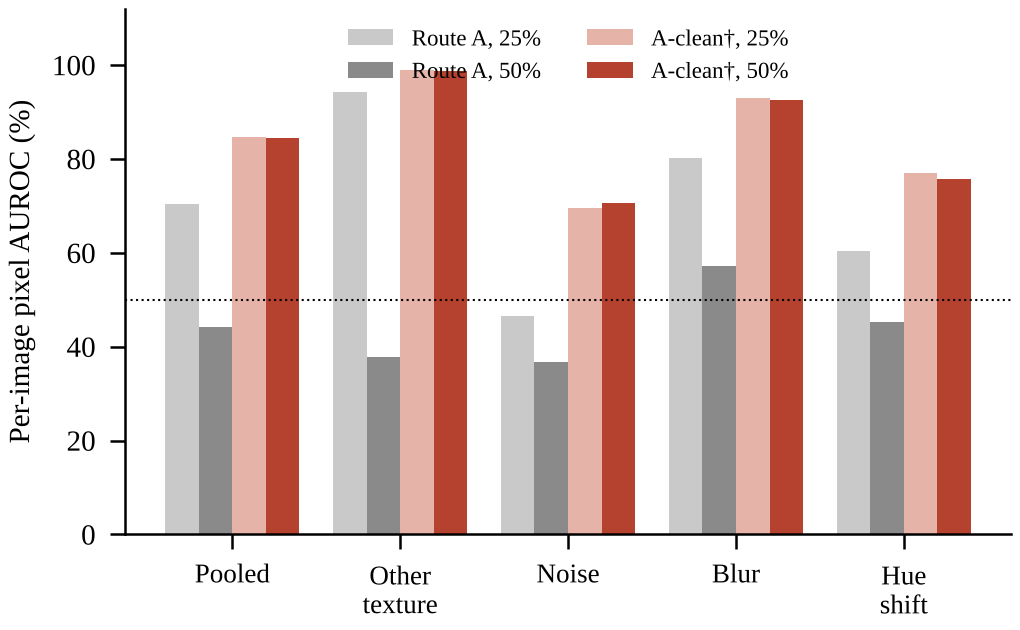
\includegraphics[width=\columnwidth]{fig4_coverage_25_50.png}
\caption{Per-image pixel AUROC at 25\% and 50\% defect coverage in the
synthetic sweep, pooled and by defect type. $^\dagger$Diagnostic only.}
\label{fig:coverage}
\end{figure}

\subsection{Negative results}
% Key points:
%  - Feature drift rises with size, but its association with AUROC at a fixed
%    size has the wrong sign (positive): not a mechanism.
%  - Routing: always-B 48.9% Pixel AP, calibrated router 26.2%, raw 16.2%;
%    best per-image choice adds at most 0.25 AUROC points in any texture.
%  - Image-level mean score: AUROC 98.0 vs 87.0, but the pre-set test holds in
%    2 textures (leather, tile), not the 4 required: not claimed.
%  - Small defects: A beats B only on leather (paired Wilcoxon, Holm
%    p = 0.004, median gain 0.18 AUROC points).
\todo{The four negative results.}

\subsection{Comparison with published methods}
% Key points: indicative only, protocols differ. Route B matches AnomalyDINO
% on AU-PRO (94.9 vs 94.9), is close to Aota, below FCA and SubspaceAD.
% Not a state-of-the-art method.
\todo{Describe Table~\ref{tab:published}.}

\begin{table}[t]
\centering
\caption{Five-texture averages (\%) as reported under each paper's own
protocol; averages for \cite{yao2025grnr}, \cite{damm2025anomalydino} and
\cite{lendering2026subspacead} computed from per-texture tables.
n/r: not reported.}
\label{tab:published}
\footnotesize
\setlength{\tabcolsep}{4pt}
\begin{tabular}{llccc}
\toprule
Method & Setting & Img.\ AUROC & Pix.\ AUROC & PRO \\
\midrule
\RA\ (ours) & 0-shot & 87.0 & 92.1 & 86.6 \\
\RB\ (ours) & 4-shot & 99.8 & 97.0 & 94.9 \\
Aota et al.\ \cite{aota2023zeroshot} & 0-shot & 99.7 & 97.5 & 93.8 \\
FCA \cite{ardelean2024highfidelity} & 0-shot & 99.6 & 98.7 & 97.2 \\
GRNR \cite{yao2025grnr} & 0-shot & 99.1 & 96.2 & n/r \\
AnomalyDINO \cite{damm2025anomalydino} & 4-shot & 99.5 & n/r & 94.9 \\
SubspaceAD \cite{lendering2026subspacead} & 4-shot & 99.9 & 98.4 & 97.2 \\
\bottomrule
\end{tabular}
\end{table}

\subsection{Feature-layer sweep}
% Key points: blocks 6, 8, 10, 12 and the mean of 7-9; 23 of 30 Route A
% variants gain at least 3 AU-PRO points; Route B improves too, so the
% same-layer AU-PRO gap falls from 8.3 to 3.1-6.9 (full) and 2.2-3.3
% (border ignored). Slope difference -1.1 to -1.7 at intermediate layers,
% all intervals exclude 0 on the full image; with the border ignored the
% mean of 7-9 just includes 0 (+0.05). Block 10: Route A image AUROC 34.7
% full vs 97.2 border ignored (border artefact). No layer chosen on the test set.
\todo{Describe Table~\ref{tab:layergap} and Table~\ref{tab:layerslope}.}

\begin{table}[t]
\centering
\caption{\RB\ minus \RA\ at the same layer (mean scoring, $1\times1$
pooling), five-texture averages in points: full image (F) and border ignored
(C; two border-only defective images dropped). \RB: mean of three seeds.}
\label{tab:layergap}
\footnotesize
\setlength{\tabcolsep}{3pt}
\begin{tabular}{llcccc}
\toprule
Layer & Prot. & Pixel AP & AU-PRO & Pix.\ AUROC & Img.\ AUROC \\
\midrule
6    & F & $+15.0$ & $+4.9$ & $+2.1$ & $+6.1$ \\
6    & C & $+6.4$  & $+2.3$ & $+0.8$ & $+2.3$ \\
8    & F & $+11.4$ & $+3.1$ & $+1.6$ & $+8.0$ \\
8    & C & $+7.2$  & $+2.5$ & $+1.0$ & $+1.1$ \\
10   & F & $+30.3$ & $+6.9$ & $+3.3$ & $+64.9$ \\
10   & C & $+3.9$  & $+2.2$ & $+1.2$ & $+2.5$ \\
12   & F & $+17.9$ & $+8.3$ & $+4.9$ & $+12.7$ \\
12   & C & $+7.5$  & $+4.0$ & $+3.0$ & $+8.5$ \\
7--9 & F & $+14.3$ & $+4.5$ & $+2.3$ & $+9.1$ \\
7--9 & C & $+8.6$  & $+3.3$ & $+1.3$ & $+1.4$ \\
\bottomrule
\end{tabular}
\end{table}

\begin{table}[t]
\centering
\caption{\RA\ (mean scoring, $1\times1$ pooling) at different DINOv2 layers:
five-texture AU-PRO (full image / border ignored) and slope difference
A $-$ B at the same layer (points per unit of log area; \RB\ seed 42).
7--9: mean of blocks 7--9.}
\label{tab:layerslope}
\footnotesize
\setlength{\tabcolsep}{3pt}
\begin{tabular}{lccc}
\toprule
Layer & AU-PRO F / C & A $-$ B, full & A $-$ B, border ignored \\
\midrule
6    & 91.2 / 93.2 & $-1.16$ [$-1.66$, $-0.69$] & $-0.47$ [$-0.92$, $-0.12$] \\
8    & 93.4 / 93.4 & $-1.12$ [$-1.67$, $-0.61$] & $-0.61$ [$-1.23$, $-0.07$] \\
10   & 89.5 / 93.3 & $-1.68$ [$-2.42$, $-0.97$] & $-0.81$ [$-1.55$, $-0.29$] \\
12   & 86.6 / 89.1 & $-2.72$ [$-3.49$, $-1.93$] & $-1.47$ [$-2.30$, $-0.85$] \\
7--9 & 92.1 / 92.7 & $-1.22$ [$-1.84$, $-0.64$] & $-0.60$ [$-1.29$, $+0.05$] \\
\bottomrule
\end{tabular}
\end{table}
      % tables and figures are ready inside
% \section{Discussion}
\label{sec:discussion}
% Course PDF: discussion = meaning, comparison, limitations.
% Points to interpret (in your words):
%  1. Why the gap grows: the defect enters the mean reference of Route A.
%     Evidence: A-clean, the contamination index, the 50% collapse.
%  2. What is NOT explained: about half of the real-defect slope remains.
%  3. The size dependence belongs to the simple mean reference, not to
%     single-image methods in general (FCA is not steeper than Route B).
%  4. Feature effect: intermediate layers raise both methods and roughly halve
%     the slope, but a significant size dependence remains at every layer on
%     the full image.
%  5. Practical meaning: what an engineer should do with large defects.
\todo{Interpretation of the findings.}

\subsection*{Limitations}
% (i) five textures, one dataset, one backbone (five layer settings, none
%     chosen on the test set); (ii) three seeds in the main table (sample SD
%     about 22% larger than the population SD shown); (iii) Route B is our
%     implementation of the AnomalyDINO idea; (iv) published numbers use other
%     protocols; (v) synthetic defects are not real defects and A-clean uses
%     the mask; (vi) border artefacts change absolute scores; (vii) Route B's
%     Pixel AP is below a published batched zero-shot result (67.3)
%     \cite{legia2025consistent}; (viii) fixed effects cannot fully separate
%     size from defect type.
\todo{Limitations.}

% \section{Conclusion}
\label{sec:conclusion}
% Course PDF: take-home message and future work. One paragraph, no new numbers
% that are not already in the Results.
%  - Take-home: mean self-similarity loses accuracy as defects grow; a few
%    clean references help; a robust single-image reference (FCA) is not
%    steeper; contamination of the image's own reference explains about half.
%  - Future work: a second texture dataset, a second backbone, a deployable
%    fix for contamination compared with FCA.
\todo{Conclusion and future work.}

% \section*{Declarations}
% Most journals require these. Keep them short and true.

\noindent\textbf{Author contributions (CRediT).}
% Each author confirms their OWN roles; the supervisor agrees the final list.
% Draft from your description:
%  Abdelilah Agouni: Conceptualization, Methodology, Software, Validation,
%   Formal analysis, Investigation, Data curation, Visualization,
%   Writing -- original draft, Writing -- review & editing.
%  Byan Hussein: Investigation, Validation, Writing -- review & editing.
%  Bilal Yousfi: Supervision.
\todo{Confirm each author's roles.}

\noindent\textbf{Use of AI tools.}
% Follow your professor's answer and the journal's policy. Facts to disclose:
% Claude and Claude Code (Anthropic) were used for analysis scripts,
% literature screening and drafting help; the authors designed the study,
% checked all outputs against the result files and are responsible for the content.
\todo{AI-use statement, in line with the professor's rules.}

\noindent\textbf{Data and code availability.}
% MVTec AD is available from its owner and is not redistributed. Code and
% results: git repository, release tag v1.0-results (commit 5c10100, branch
% main), commands in REPRODUCE.md. FCA: commit afe8326 of the public
% repository (MIT licence).
\todo{Add the repository URL when it is public.}

\noindent\textbf{Ethics.} \todo{Confirm with the university whether a statement is required.}
% Public benchmark images only; no human or animal participants; no personal data.

\noindent\textbf{ORCID iDs.} Abdelilah Agouni: 0009-0005-0521-3798.
\todo{Byan Hussein and Bilal Yousfi.}

\noindent\textbf{Funding.} \todo{``This research received no external funding.'' -- confirm.}

\noindent\textbf{Conflicts of interest.} \todo{``The authors declare no conflict of interest.'' -- confirm with all authors.}

\noindent\textbf{Thesis disclosure.}
% Course PDF: papers based on your thesis are acceptable if you disclose it.
\todo{State that this paper is based on the first author's MSc thesis.}


\printbibliography

\end{document}

% =====================================================================
% CITATION KEYS (all verified, with DOIs, in refs.bib)
%   bergmann2021mvtec          MVTec AD dataset (IJCV 2021)
%   aota2023zeroshot           Aota et al., zero-shot texture AD (WACV 2023)
%   ardelean2024highfidelity   FCA (WACV 2024)
%   yao2025grnr                GRNR (IEEE TSMC: Systems 2025)
%   zhang2025nlpa              NLPA-AD (Applied Intelligence 2025)
%   roth2022patchcore          PatchCore (CVPR 2022)
%   damm2025anomalydino        AnomalyDINO (WACV 2025)
%   lendering2026subspacead    SubspaceAD (CVPR 2026, accepted)
%   li2024musc                 MuSc (ICLR 2024)
%   legia2025consistent        CoDeGraph / consistent anomalies (arXiv 2025)
%   lehr2024limitations        Defect-size limits of AD (SPIE ICMV 2023)
%   villanueva2026cleaning     Contaminated reference sets (Electronics 2026)
%   oquab2024dinov2            DINOv2 (TMLR 2024)
% Also in refs.bib, not cited yet: luo2025inp, bergmann2019mvtec,
%   jeong2023winclip, zagoruyko2016wide.
% =====================================================================
